%UNIT 5: UNIQUENESS OF SOLUTIONS	
%%%%%%%%%%%%%%%%%%%%%%%%%%%
%%%% Put the following at the top of each .tex file  %
\pagestyle{fancy}
\renewcommand{\theUnit}{5}
\ifthenelse{\isundefined{\UnitPageNumbers}}{}{\setcounter{page}{1}}
\rhead{Unit \theUnit: Uniqueness of Solutions}
\lhead{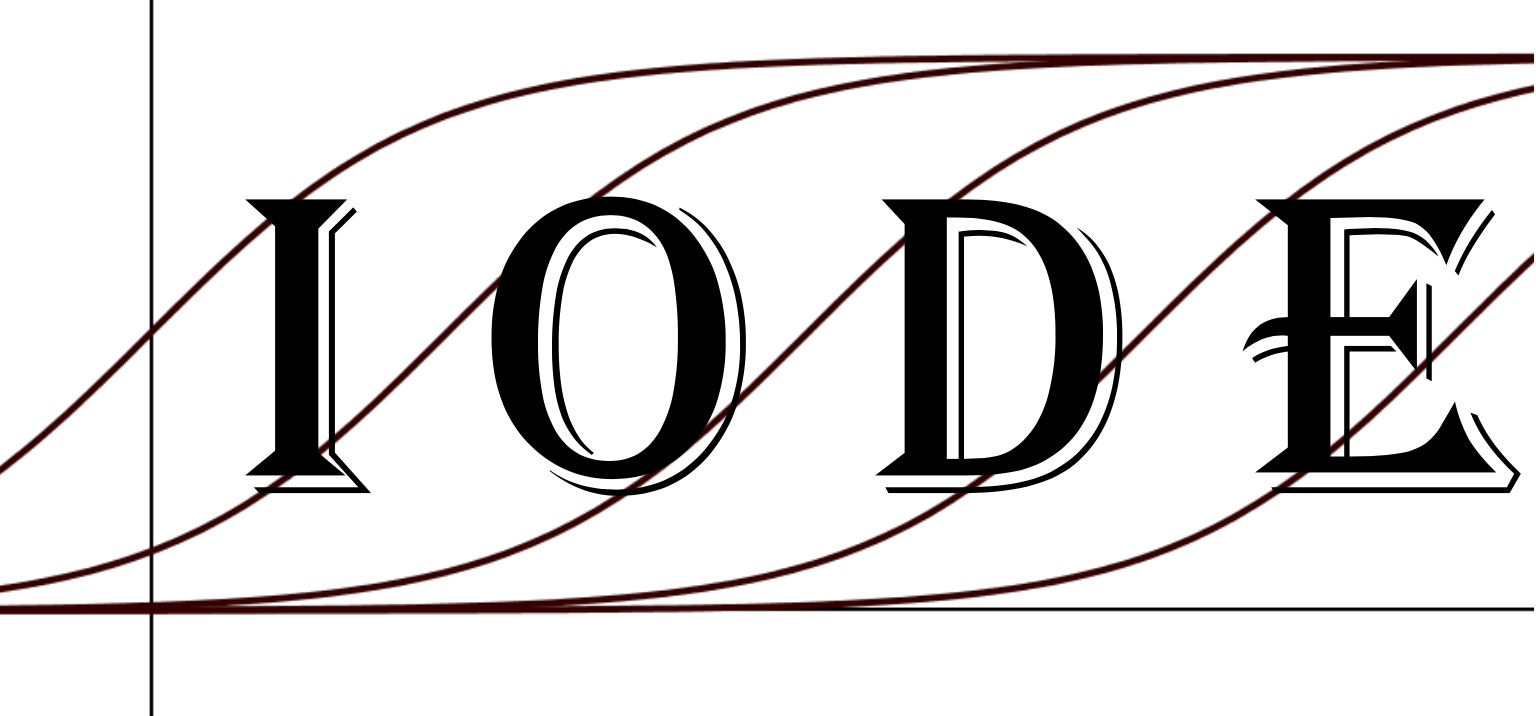
\includegraphics[width=1.25cm]{IODE-logo.png}}
\rfoot{\mypage}
\lfoot{}
\cfoot{}
\fancypagestyle{firstfooter}{\footskip = 50pt}
\renewcommand{\footrulewidth}{.4pt}
%%%%%%%%%%%%%%%%%%%%%%%%%%%
\vspace*{-20pt} \thispagestyle{firstfooter}
\pagebegin{Proposed Paths of Descent}

A group of scientists at the Federal Aviation Association has come up with the following two different rate of change equations to predict the height of a helicopter as it nears the ground: 
\[ \frac{dh}{dt}=-h \qquad \text{ and } \qquad \frac{dh}{dt}=-h^{\frac{1}{3}}\]
 
For both rate of change equations $h$ is in feet and $t$ is in minutes. The scientists, of course, want their models to predict that a helicopter actually lands - but do either or both of the proposed models predict this? 
\begin{enumerate}
\item Getting familiar with the differential equations: \label{05problem1}

\begin{enumerate}
\item Just by examining the rate of change equations, what can you say about the height of the helicopter as predicted by $\displaystyle\frac{dh}{dt}=-h$  and by $\displaystyle\frac{dh}{dt}=-h^{\frac{1}{3}}$? More specifically, as $h$ approaches zero, what can you say about $\displaystyle\frac{dh}{dt}$ and what does that imply about whether the model predicts that the helicopter lands? \label{05problem1parta}
\vfill

\item Sketch your best guess for a height versus time solution graph for each rate of change equation. \label{05problem1partb}
\end{enumerate}
\vfill

\item	\label{05problem2}
\begin{enumerate}
\item What do each of the proposed rate of change equations say about the solution to the differential equation if the helicopter is already on the ground? Explain and sketch a corresponding graph of height versus time on the same set of axes from part \ref{05problem1partb}. \label{05problem2parta}
\vfill

\item Interpret the initial condition $h(0) = 0$, and explain why $h(t) = 0$ should be a solution to each differential equation under this initial condition. \label{05problem2partb}
\vfill
\end{enumerate}

\clearpage

\item Use the Geogebra applet, \href{https://ggbm.at/dJsACfAN}{\underline{https://ggbm.at/dJsACfAN}}, to investigate the slope fields. What do the slope fields suggest about whether the model predicts if the helicopters will land?  How do the slope fields compare with your sketches from part \ref{05problem1partb}? \label{05problem3}

\vspace{-.05in}\hspace{-.5in}
\includegraphics[width=0.5in]{05/05ProposedPathsQR.png}
\vfill

\item Solve the following initial value problems: \label{05problem4}

\begin{enumerate}
\item $\displaystyle\frac{dh}{dt}=-h$

\begin{hnumerate}
\hitem $h(0) = 2$
\hitem $h(0) = 0$ (\textit{Hint}: Use problem \ref{05problem2partb}) \hspace{1in}
\end{hnumerate}
\vfill

\item $\displaystyle\frac{dh}{dt}=-h^{\frac{1}{3}}$
  			                                    
\begin{hnumerate}
\hitem $h(0) = 2$
\hitem $h(0) = 0$ (\textit{Hint}: Use problem \ref{05problem2partb}) \hspace{1in}
\end{hnumerate}
\end{enumerate}
\vfill

\item
\begin{enumerate}
\item For each differential equation, interpret the results from problem \ref{05problem4} in terms of whether the model predicts the helicopter will ever touch the ground. If so, at what time? \label{05problem5parta}
\vfill

\item For each differential equation, interpret the results from problem \ref{05problem4} in terms of whether graphs of (i) and (ii) will ever touch or cross. \label{05problem5partb}
\vfill
\end{enumerate}

\clearpage

\item	One difference between the two differential equations is the partial derivative of the right hand side at $h = 0$. That is,
\[
\frac{\partial f}{\partial h}, \quad \text{where } f(h)=-h
\]
for one differential equation is different than
\[
\frac{\partial f}{\partial h}, \quad \text{where } f(h)=-h^{\frac{1}{3}}
\]
for the other differential equation. \\
\vs
Accurately draw graphs of $\displaystyle\frac{dh}{dt}$ versus $h$ for both differential equations and use these graphs to determine the partial derivatives at $h = 0$ for each differential equation. \label{05problem6}
\end{enumerate}
\vfill

\clearpage

\pagebegin{The Uniqueness Theorem}

In the formal language of differential equations, the term ``unique'' or ``uniqueness'' refers to whether or not two solution functions ever touch or cross each other. Using this terminology, the two solutions you found to $\displaystyle\frac{dh}{dt}=-h$ are unique while the two solutions you found to $\displaystyle\frac{dh}{dt}=-h^{\frac{1}{3}}$ are not unique. Fortunately, one does not have to always analytically solve a differential equation to determine if solutions will or will not be unique. There is a theorem, the \textbf{Uniqueness Theorem}, which sets out conditions for when solutions are unique. \\

\textbf{Theorem.} Let $f(x,y)$ be a real valued function which is continuous on the rectangle 
\[R=\{(x,y):|x-x_0 |\leq a,|y-y_0 |\leq b\}.\]
Assume $f$ has a partial derivative with respect to $y$ and that this partial derivative $\partial f/\partial y$ is also continuous on the rectangle $R$. Then there exists an interval 
\[I = [x_0 - h, x_0 + h] \text{ (with $h \leq a$)}\]
such that the initial value problem 
\[ \frac{dy}{dx}=f(x,y), \qquad y(x_0)=y_0\]
has a unique solution $y(x)$ defined on the interval $I$.
\vspace{.25in}

\begin{enumerate}[resume]
\item	Explain how the conditions of this theorem relate to solutions of $\displaystyle\frac{dh}{dt}=-h$. \label{05problem7}
\vfill

\item	If you are given a differential equation and determine that the conditions of the uniqueness theorem are NOT met in a specific range of $y$-values, what can you conclude about the graphs of solution functions within that range of $y$-values? Explain. \label{05problem8}
\vfill
\end{enumerate}

\clearpage

%%%%%%%%%%%%%%%%%%%%%%%%%%%%%%%%%%%%%%
\pagebegin{Homework Set 5}

\begin{enumerate}
\item Suppose two planes start descending at the same time, one is directly above the other and both follow the same differential equation, $\displaystyle\frac{dh}{dt}=-h^{1/3}$. Is there any possibility of a midair collision? Will the initially higher one ever get below the initially lower one? Develop two different arguments to support your conclusion, one based on the uniqueness theorem and one based on the fact this differential equation is autonomous and hence graphs of solutions are related to each in a particular way. \label{05HWproblem1}

\item In light of the \textbf{Uniqueness Theorem}, consider the population model \label{05HWproblem2} 
\[
\frac{dP}{dt}=0.3P\left(1-\frac{P}{12.5}\right).
\]
If $P(0) < 12.5$, will the population ever reach 12.5? Explain.

\item For each differential equation, determine (with reasons) whether or not graphs of solution functions will ever touch any and all equilibrium solution functions (consider both positive and negative values of $t$). \label{05HWproblem3}

\[
\text{(a) } \frac{dL}{dt}=.5(1-L) \hspace{.35in}\text{(b) } \frac{dy}{dt}=0.3y\left(1-\frac{y}{10}\right) \hspace{.35in} \text{(c) } \frac{dy}{dt}=-t+1 \hspace{.35in} \text{(d) } \frac{dy}{dt}=y^{\frac{1}{2}}
\]

\item	Suppose two students are memorizing a list according to the same model  $\displaystyle \frac{dL}{dt}=0.5(1-L)$  where $L$ represents the fraction of the list that is memorized at any time $t$. According to the uniqueness theorem, will the student who starts out knowing none of the list ever catch up to the student who knows one-third of the list? Explain. \label{05HWproblem4}

\item	What values of $p$ result in predictions that the helicopter will land in a finite amount of time for the model $\displaystyle\frac{dh}{dt} = -h^p$? Explain and show all work. \label{05HWproblem5}

\end{enumerate}


